% Compile from the repository root:
% pdflatex -interaction=nonstopmode -halt-on-error -output-directory=docs/relatorio docs/relatorio/relatorio-projeto-g2.tex
% Run twice to resolve cross-references. Pages 1--5 are the report; page 6 is references.
\documentclass[a4paper,11pt]{article}
\usepackage[T1]{fontenc}
\usepackage[utf8]{inputenc}
\usepackage[british]{babel}
\usepackage[margin=22mm,headheight=14pt,headsep=7mm,footskip=10mm]{geometry}
\usepackage{lmodern}
\usepackage{microtype}
\usepackage{amsmath,amssymb,mathtools}
\usepackage{graphicx,booktabs,array}
\usepackage[font=small,labelfont=bf]{caption}
\usepackage{xcolor}
\usepackage{fancyhdr}
\usepackage{enumitem}
\usepackage{titlesec}
\usepackage[colorlinks=true,linkcolor=black,citecolor=black,urlcolor=blue!45!black]{hyperref}
\definecolor{ink}{HTML}{17334B}
\titleformat{\section}{\large\bfseries\color{ink}}{\thesection}{0.6em}{}
\titleformat{\subsection}{\normalsize\bfseries\color{ink}}{\thesubsection}{0.6em}{}
\titlespacing*{\section}{0pt}{10pt}{5pt}
\titlespacing*{\subsection}{0pt}{8pt}{4pt}
\setlength{\parindent}{0pt}
\setlength{\parskip}{5pt}
\setlength{\abovedisplayskip}{6pt plus 1pt minus 1pt}
\setlength{\belowdisplayskip}{6pt plus 1pt minus 1pt}
\setlength{\textfloatsep}{9pt}
\setlength{\intextsep}{9pt}
\setlength{\tabcolsep}{6pt}
\setlist{nosep,leftmargin=*}
\pagestyle{fancy}
\fancyhf{}
\fancyhead[L]{\small\color{ink}Learning the metric of a $\mathrm{G}_2$-structure}
\fancyhead[R]{\small MM845}
\fancyfoot[C]{\small\thepage}
\renewcommand{\headrulewidth}{0.3pt}
\newcommand{\R}{\mathbb{R}}
\newcommand{\Gtwo}{\mathrm{G}_2}
\newcommand{\SO}{\mathrm{SO}}
\newcommand{\GLp}{\mathrm{GL}^{+}}
\newcommand{\SPD}{\operatorname{Sym}^{+}}
\newcommand{\Fhat}{\widehat F}
\newcommand{\normF}[1]{\left\lVert#1\right\rVert_{\mathrm F}}
\graphicspath{{docs/relatorio/relatorio-assets/}{relatorio-assets/}}
\IfFileExists{docs/relatorio/relatorio-assets/results-summary.tex}
  {\input{docs/relatorio/relatorio-assets/results-summary.tex}}
  {% Generated from outputs/full/metrics.csv; do not edit numeric entries by hand.
\newcommand{\accuracyrows}{
Ridge & $36.58\pm0.00$ & 48.29 & $62.29\pm0.00$ & 72.86 \\
MLP & $25.81\pm0.09$ & 33.92 & $43.57\pm0.08$ & 64.60 \\
MLP + rotations & $24.99\pm0.07$ & 33.25 & $42.79\pm0.01$ & 62.87 \\
}
\newcommand{\geometryrows}{
Ridge & $0.0152\pm0.0000$ & $0.2123\pm0.0000$ & $0.0132\pm0.0000$ & $0.1459\pm0.0000$ \\
MLP & $0.2355\pm0.0016$ & $0.2658\pm0.0029$ & $0.2985\pm0.0057$ & $0.3244\pm0.0027$ \\
MLP + rotations & $0.2223\pm0.0021$ & $0.2519\pm0.0028$ & $0.2817\pm0.0078$ & $0.3118\pm0.0044$ \\
}
\newcommand{\IDAccuracyGain}{3.18}
\newcommand{\IDEquivarianceGain}{5.61}
\newcommand{\IDPlainScaleFourError}{104.9}
\newcommand{\IDAugmentedScaleFourError}{103.0}
\newcommand{\OODAccuracyGain}{1.78}
\newcommand{\OODEquivarianceGain}{5.61}
\newcommand{\OODPlainScaleFourError}{172.3}
\newcommand{\OODAugmentedScaleFourError}{168.2}
}
\hypersetup{pdftitle={Learning the metric induced by a G2-structure},
            pdfauthor={Eduardo Toffolo},pdfsubject={MM845 project report}}

\begin{document}
\thispagestyle{plain}
{\LARGE\bfseries\color{ink}Learning the metric induced\par
by a $\Gtwo$-structure\par}
\vspace{4pt}
{\large Generalisation and equivariance through rotation augmentation\par}
\vspace{5pt}
Eduardo Toffolo \hfill University of Campinas\par
{\small MM845 --- AI for Geometry}\par
{\small Code and reproduction instructions:
\url{https://github.com/EToffolo/AI-Project}}\par

\vspace{5pt}
\textbf{Abstract.}
A positive $3$-form in seven dimensions determines a unique metric through a known
algebraic formula. This project tests how accurately a generic neural regressor
learns that map and whether rotating both inputs and targets improves its geometric
behaviour. Exact synthetic labels allow separate tests of prediction, equivariance
and homogeneity. With 21,000 training examples, rotation augmentation reduces the
mean seed-wise median relative error from 25.81\% to 24.99\% in distribution and
from 43.57\% to 42.79\% under extrapolation. Rotation defects also decrease, but
remain substantial. The results support a modest benefit from augmentation while
showing the limits of learning mathematical structure without imposing it.

\section{Introduction and related work}
A $\Gtwo$-structure encodes a metric using a differential $3$-form. Its pointwise
linear algebra is explained by Karigiannis~\cite{karigiannis}; Grigorian~\cite{grigorian}
gives explicit metric formulas in the study of deformations. Here the problem is
restricted to one oriented vector space. There are no differential equations or
torsion-free conditions. The known formula makes this a controlled benchmark for
learning a nonlinear tensor-valued map.

Symmetry provides a natural inductive bias. Cohen and Welling~\cite{cohen} construct
layers that enforce group equivariance, whereas Chen, Dobriban and Lee~\cite{chen}
interpret augmentation as averaging over group orbits and analyse variance reduction.
Their results motivate the experiment; they do not guarantee equivariance of the
generic regressor used here. The question is whether $\SO(7)$ augmentation reduces
rotation defects without materially degrading accuracy, under a fixed training protocol.

\section{Mathematical background}
Let $V=\R^7$ with dual basis $e^1,\ldots,e^7$, orientation
$\mathrm{vol}_0=e^1\wedge\cdots\wedge e^7$, and $e^{ijk}=e^i\wedge e^j\wedge e^k$.
Use the reference form
\begin{equation}
\varphi_0=e^{123}+e^{145}+e^{167}+e^{246}-e^{257}-e^{347}-e^{356}.
\end{equation}
The positive orbit is $\mathcal P=\{A^*\varphi_0:A\in\GLp(7)\}$, where
$(A^*\varphi)(u,v,w)=\varphi(Au,Av,Aw)$ and $\GLp(7)$ denotes positive-determinant
invertible matrices. Its stabiliser is $\Gtwo\subset\SO(7)$, so
$F:\mathcal P\to\SPD(7)$ is well defined by $F(A^*\varphi_0)=A^\top A$.
$\SPD(7)$ is the set of symmetric positive-definite $7\times7$ matrices.

In this orientation convention~\cite{grigorian}, the exact formula is
\begin{equation}\label{eq:exact}
B_{ij}(\varphi)\,\mathrm{vol}_0
=\tfrac16(\iota_{e_i}\varphi)\wedge(\iota_{e_j}\varphi)\wedge\varphi,
\qquad F(\varphi)=(\det B)^{-1/9}B,
\end{equation}
where $\iota_{e_i}$ contracts a form with $e_i$. Indeed,
$B=g_\varphi\sqrt{\det g_\varphi}$ implies $\det B=(\det g_\varphi)^{9/2}$.
Naturality and cubic dependence of $B$ give the identities
\begin{equation}\label{eq:identities}
F(C^*\varphi)=C^\top F(\varphi)C\quad(C\in\GLp(7)),\qquad
F(t\varphi)=t^{2/3}F(\varphi)\quad(t>0).
\end{equation}
These identities are diagnostics for the learned map, rather than constraints built
into its architecture. In particular, the target transforms under rotations; it is
not an invariant scalar label.

\newpage
\section{Data generation and experimental design}
Draw independent Haar rotations $Q_1,Q_2\in\SO(7)$ using Gaussian QR with sign and
determinant corrections, and independent log singular values $s_i$. Generate
\begin{equation}\label{eq:data}
A=Q_1\operatorname{diag}(e^{s_1},\ldots,e^{s_7})Q_2,
\qquad (\varphi,g)=(A^*\varphi_0,A^\top A).
\end{equation}
The learner receives only the 35 coefficients $\varphi_{ijk}$, $i<j<k$, in
lexicographic order; no $3!$ rescaling is used. It never receives $A$ or $s$.
The eigenvalues of $g$ are $e^{2s_i}$. Thus generation guarantees positivity and
provides exact labels independently of the exterior-algebra implementation of
Eq.~\eqref{eq:exact}.

For the in-distribution (ID) population, $s_i\sim U[-0.35,0.35]$. A single dataset
of 30,000 pairs, generated with seed 2026, is randomly split into 21,000 training,
4,500 validation and 4,500 test sources. A separate out-of-distribution (OOD) test
contains 4,500 pairs with $s_i\sim U[-0.7,0.7]$, conditioned on
$\max_i|s_i|>0.35$. This shifts singular values beyond the training range, rather
than merely choosing new rotations. Metric eigenvalues lie in approximately
$[0.497,2.014]$ for ID and $[0.247,4.055]$ for OOD; the corresponding upper bounds
on the spectral condition number are $e^{1.4}\approx4.06$ and $e^{2.8}\approx16.44$.

Splitting precedes augmentation. Transformed copies inherit their source split,
preventing leakage between training and held-out data. Inputs are standardised
coefficient by coefficient using training-only means and standard deviations;
per-sample norms are retained. Nested training subsets of 2,100, 7,000 and 21,000
examples are shared by all methods within each seed (11, 22 and 33). At the largest
size, the three seeds use the same full training set. Validation and test sets are
fixed, so seed variation measures training variation, not uncertainty over new datasets.

The source population is already rotation invariant: replacing $A$ by $AQ$ leaves
its distribution unchanged because $Q_2Q$ remains Haar. Augmentation therefore
provides new orientations of a finite sample, without expanding population support.
Float64 label checks compare Eq.~\eqref{eq:exact}, using only $\varphi$, with
$A^\top A$ on 64 randomly selected ID and 64 OOD pairs. The maximum relative
discrepancy is $5.61\times10^{-16}$; $F(\varphi_0)=I$ is also verified.

\section{Learning methods}
\textbf{Ridge baseline.}
An affine map predicts the 28 independent entries of a symmetric matrix, without
enforcing positivity. It minimises squared errors of those entries plus an
$\ell_2$ penalty on weights. An unpenalised intercept is included. The penalty is
chosen from $\{10^{-4},10^{-2},1,10^2,10^4\}$ using validation relative loss.

\textbf{Neural regressors.}
The architecture is a $35$--$128$--$128$--$28$ multilayer perceptron (MLP) with two
ReLU hidden layers. Its outputs form a lower triangular matrix $L$: off-diagonal
entries are unrestricted, and diagonal entries are
$\operatorname{softplus}(z)+10^{-5}$. The prediction is $\Fhat(\varphi)=LL^\top$,
ensuring symmetry and positivity in exact arithmetic. Both MLPs minimise
\begin{equation}\label{eq:loss}
\mathcal L=\frac1m\sum_{a=1}^{m}
\frac{\normF{\Fhat(\varphi_a)-g_a}^{2}}{\normF{g_a}^{2}},
\end{equation}
with Adam~\cite{adam}, learning rate $10^{-3}$ and batch size 256. The maximum is
100 epochs; early stopping uses patience 15 and improvement threshold $10^{-5}$.
The checkpoint with the smallest validation loss is restored.

The augmented MLP draws a fresh independent Haar rotation per example per minibatch
and trains on $(Q^*\varphi,Q^\top gQ)$, before input standardisation. Initial
weights and minibatch orders match the ordinary MLP within each seed; rotation
randomness uses a separate stream. Maximum epochs and optimiser settings match,
although actual epochs and computation may differ. All 27 fitted models
(9 ridge, 18 MLP) run on CPU. Test data do not select hyperparameters or checkpoints.

\newpage
\section{Results and analysis}
\subsection{Predictive accuracy and sample size}
For each held-out pair define the relative Frobenius error
\begin{equation}\label{eq:error}
E(\varphi,g)=\frac{\normF{\Fhat(\varphi)-g}}{\normF{g}},
\qquad \normF{M}^{2}=\sum_{i,j}M_{ij}^{2}.
\end{equation}
This measures error of the entire matrix, counting off-diagonal entries twice.
A 25\% error is not a classification failure rate. Unlike the training loss in
Eq.~\eqref{eq:loss}, the statistics below are not squared.

\begin{table}[h]
\centering
\caption{Predictive errors (\%) at $n=21{,}000$. Medians: mean $\pm$ sample standard
deviation over three seeds. p95: mean of seed-wise 95th percentiles.}
\label{tab:accuracy}
\small
\begin{tabular}{@{}lrrrr@{}}
\toprule
&\multicolumn{2}{c}{ID: 4,500 examples}&\multicolumn{2}{c}{OOD: 4,500 examples}\\
\cmidrule(lr){2-3}\cmidrule(l){4-5}
Model&Median&p95&Median&p95\\
\midrule
\accuracyrows
\bottomrule
\end{tabular}
\end{table}

The MLP's median error is about 29\% lower than ridge on ID and 30\% lower on OOD.
Augmentation adds a smaller gain: \IDAccuracyGain\% relative to the plain MLP on ID
and \OODAccuracyGain\% on OOD, or about 0.82 and 0.78 percentage points.
Each seed improves, but errors remain high.

\begin{figure}[h]
\centering
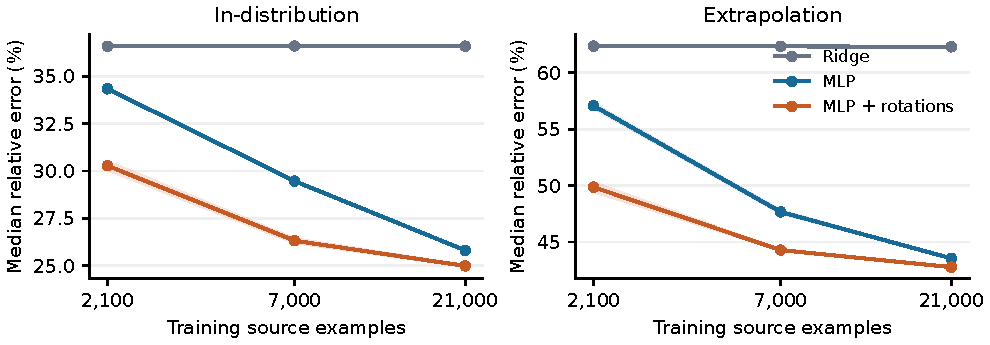
\includegraphics[width=\textwidth]{learning-curves.pdf}
\caption{Median predictive error versus source sample size. Lines average seed-wise
medians; shading is $\pm$ one sample standard deviation, not a confidence interval.}
\label{fig:learning}
\end{figure}

Larger datasets improve the neural regressors (Figure~\ref{fig:learning}), while
ridge stays close to 36.6\% ID and 62.3\% OOD. At 2,100 sources, augmentation
changes the mean median from 34.34\% to 30.28\% ID and from 57.08\% to 49.87\% OOD:
relative gains of approximately 11.8\% and 12.6\%. The declining gain suggests
augmentation is most useful when finite samples cover orientations sparsely;
the curves do not isolate that explanation causally.

Extrapolation remains much harder. For the augmented MLP, the OOD median is
42.79\%, versus 24.99\% ID, and the OOD p95 reaches 62.87\%. Rotations preserve
the singular values of $A$ and cannot directly expose the learner to the broader
OOD singular-value range. The gain therefore does not establish reliable
extrapolation to arbitrary scales or conditioning.

All methods have zero non-positive-definite predictions on the base ID and OOD
tests: at the largest size, zero failures in 13,500 predictions per method and
domain across seeds. Ridge has no positivity guarantee; the MLP guarantee holds
in exact arithmetic, so numerical failures are explicitly counted.

\newpage
\subsection{Equivariance and homogeneity}
On 512 fixed randomly selected sources per domain, evaluate the covariance defect
for fresh transformations $C$:
\begin{equation}\label{eq:defect}
D_C(\varphi,g)=
\frac{\normF{\Fhat(C^*\varphi)-C^\top\Fhat(\varphi)C}}
     {\normF{C^\top gC}}.
\end{equation}
The denominator uses the exact transformed metric. Rotations are Haar draws;
$\GLp(7)$ transformations use Eq.~\eqref{eq:data} with log bound 0.2. Indices and
transformations are shared across methods and seeds. Transformed inputs may leave
their source domain's singular-value range.

\begin{table}[h]
\centering
\caption{Geometric defects at $n=21{,}000$: mean $\pm$ sample standard deviation
of seed-wise medians. All values are dimensionless.}
\label{tab:geometry}
\small\setlength{\tabcolsep}{4pt}
\begin{tabular}{@{}lcccc@{}}
\toprule
&\multicolumn{2}{c}{ID sources}&\multicolumn{2}{c}{OOD sources}\\
\cmidrule(lr){2-3}\cmidrule(l){4-5}
Model&$\SO(7)$&$\GLp(7)$&$\SO(7)$&$\GLp(7)$\\
\midrule
\geometryrows
\bottomrule
\end{tabular}
\end{table}

Augmentation reduces the mean rotation median by \IDEquivarianceGain\% ID and
\OODEquivarianceGain\% OOD. The declared criterion requires a smaller rotation
median in each seed and domain, allowing at most a 5\% relative increase in
predictive median at the largest size. All six comparisons satisfy it, with
improved accuracy. $\GLp(7)$ defects also decline. Three seeds and shared tests
do not establish statistical significance or exact equivariance.

Ridge illustrates a pitfall: for seed 11, its mean ID prediction is close to
$1.08288I$, with only about 1.12\% mean relative variation. A constant map
$\Fhat(\varphi)=cI$ has zero rotation defect, since $Q^\top(cI)Q=cI$, while predicting
the wrong metric. Accuracy and covariance must be assessed together.

For $t\in\{0.25,0.5,2,4\}$, define a homogeneity defect and a scaled prediction error:
\begin{equation}\label{eq:scaling}
H_t=\frac{\normF{\Fhat(t\varphi)-t^{2/3}\Fhat(\varphi)}}
               {\normF{t^{2/3}g}},
\qquad E_t=\frac{\normF{\Fhat(t\varphi)-t^{2/3}g}}{\normF{t^{2/3}g}}.
\end{equation}
\begin{figure}[h]
\centering
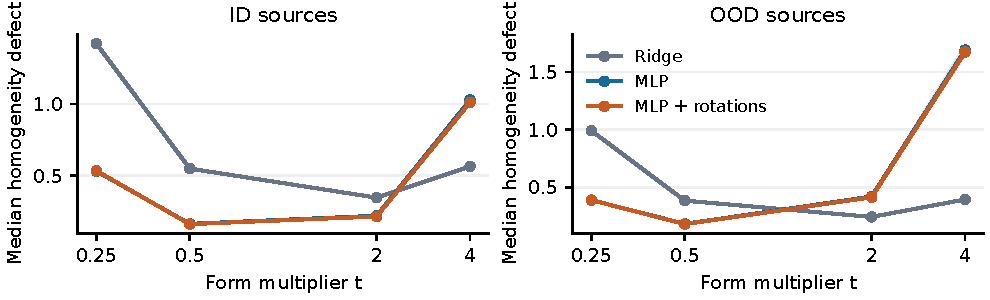
\includegraphics[width=\textwidth]{homogeneity.pdf}
\caption{Homogeneity defects on 512 sources per domain, aggregated as in
Figure~\ref{fig:learning}. Nearly overlapping MLP curves show little effect of rotations on scaling.}
\label{fig:homogeneity}
\end{figure}

At $t=4$, augmentation changes mean median $E_t$ from
\IDPlainScaleFourError\% to \IDAugmentedScaleFourError\% ID and from
\OODPlainScaleFourError\% to \OODAugmentedScaleFourError\% OOD.
Both MLPs fail severely; rotations do not enforce the degree-$2/3$ law.

\newpage
\section{Discussion, conclusion and extensions}
\textbf{Why are the errors still large?}
Labels are exact, so the discrepancy comes from approximation, optimisation and
generalisation. The map involves cubic contractions followed by determinant
normalisation, beyond the expressive scope of an affine regressor. The MLP is a
generic approximator with no built-in homogeneity or equivariance. More data help,
but the experiment does not isolate whether capacity, optimisation budget or
coverage of the 35-dimensional input domain is the main bottleneck.

\begin{figure}[h]
\centering
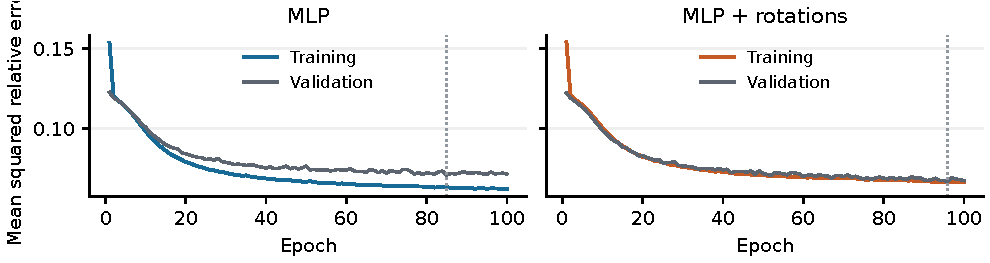
\includegraphics[width=0.94\textwidth]{training-curves.pdf}
\caption{Training and validation loss for 21,000 sources, seed 11. Dotted lines
mark selected checkpoints. Augmented training uses changing rotated samples;
validation always uses the original fixed sources.}
\label{fig:training}
\end{figure}

The nearby training and validation curves (Figure~\ref{fig:training}) suggest no
large ID generalisation gap. Augmented models select epochs 96, 98 and 97, near
the maximum of 100: compatible with limited capacity or insufficient optimisation,
without proving either. Mean measured training time is 18.9 seconds for the plain
MLP and 39.3 seconds with augmentation on the recorded CPU environment.
Equal maximum epochs do not mean equal time; early stopping may give different
update budgets. No speed comparison with the exact formula was performed.

\textbf{Conclusions.}
Neural models are more accurate than ridge, and rotation augmentation consistently
improves prediction and rotation defects under this protocol. The benefit is
strongest at smaller sample sizes and modest at the largest size. Median errors
near 25\% ID and 43\% OOD and substantial geometric defects prevent treating the
learned map as a precise replacement for the formula. Positivity, accuracy,
equivariance and homogeneity are separate properties: observing one does not
establish the others. The scope is a bounded pointwise benchmark; global
manifolds, torsion-free structures and near-singular limits remain unexplored.

\textbf{Extensions.}
First test whether the network can deliberately overfit 128--256 sources; then
compare larger architectures and longer training with validation-only selection.
An exact homogeneity constraint is possible: for
$r=\lVert\varphi\rVert_2>0$, use
$\Fhat(\varphi)=r^{2/3}h(\varphi/r)$. This preserves scale while making the identity
automatic. A further comparison should use an $\SO(7)$-equivariant tensor
architecture or features based on the contractions defining $B$. To study a
broader range of singular values, expand training support and reserve a new
external range as an independent OOD test. These are proposed experiments,
not results obtained here; observed test scores should not guide retrospective
hyperparameter selection.

\textbf{Reproducibility and use of AI.}
The repository linked on page 1 includes environment instructions and
\texttt{configs/full.json}. From its root, after activating the documented environment:
\begin{quote}\small
\verb|python -m g2metric run --config configs/full.json --output outputs/repro|
\end{quote}
A new output directory regenerates data, all 27 fits, metrics, figures and
checkpoints. Raw run outputs are excluded
from Git; this report includes the central results. Saved manifests record seeds,
versions and hashes. All 24 automated tests and the smoke pipeline pass.
Codex assisted implementation, experiments, analysis and drafting. Checks include
independent exterior-algebra labels, pullback identities, source separation and
checkpoint persistence. The author remains responsible for reviewing the submission.

\newpage
\begin{thebibliography}{9}
\bibitem{karigiannis}
S. Karigiannis.
\emph{Introduction to $\Gtwo$ geometry}.
Lecture notes, 2019; revised 2020.
\href{https://arxiv.org/abs/1909.09717}{arXiv:1909.09717}.

\bibitem{grigorian}
S. Grigorian.
\emph{Deformations of $\Gtwo$-structures with torsion}.\par
\emph{Asian Journal of Mathematics}, 20(1):123--155, 2016.\par
\href{https://arxiv.org/abs/1108.2465}{arXiv:1108.2465};
\href{https://doi.org/10.4310/AJM.2016.v20.n1.a6}{doi:10.4310/AJM.2016.v20.n1.a6}.

\bibitem{cohen}
T. S. Cohen and M. Welling.
\emph{Group equivariant convolutional networks}.
Proceedings of the 33rd International Conference on Machine Learning,
PMLR 48:2990--2999, 2016.
\url{https://proceedings.mlr.press/v48/cohenc16.html}.

\bibitem{chen}
S. Chen, E. Dobriban and J. H. Lee.
\emph{A group-theoretic framework for data augmentation}.
Journal of Machine Learning Research, 21(245):1--71, 2020.
\url{https://jmlr.org/papers/v21/20-163.html}.

\bibitem{adam}
D. P. Kingma and J. Ba.
\emph{Adam: A method for stochastic optimization}.
International Conference on Learning Representations, 2015.
\href{https://arxiv.org/abs/1412.6980}{arXiv:1412.6980}.
\end{thebibliography}
\end{document}
